%% Requires compilation with XeLaTeX or LuaLaTeX
\documentclass[10pt,xcolor={table,dvipsnames},t]{beamer}
\usetheme{UCBerkeley}
\usepackage{tikz}
\usepackage{graphicx}
\usepackage{amsmath,amsthm,amssymb}
\usepackage{physics}
\usepackage{float}
\usepackage{comment}
\usepackage{tikz-cd}
\usepackage{setspace}
\usepackage{makecell}

\title[Your Short Title]{From Quasars to Quarks: Day 1.2}
\subtitle{Classical Mechanics}
\author{Charlie Cummings \& Shaunak Modak}
\institute{tinyurl.com/FQ2Q-mechanics}
\date{September 2, 2020}

\begin{document}

\begin{frame}
    \titlepage
\end{frame}

\begin{frame}{Announcements}
    \begin{itemize}
        \item Homework 1 due Wednesday, 9/9 at 2 PM Pacific Time
        \item Lecture Wednesday and Friday next week (will record as usual)
        \item Ask questions in the chat and one of us will answer!
    \end{itemize}
\end{frame}

% Uncomment these lines for an automatically generated outline.
\begin{frame}{Outline}
    \tableofcontents
\end{frame}

\section{Math Review}

\subsection{Special Matrices}

\begin{frame}{Math Review: Special Matrices}
    % include basic recap of what a matrix is (components as a hint for vector space problem)
    % trace
    % transposes/daggers
    % define unitary and Hermitian matrices
\end{frame}

\subsection{Einstein Notation}

\begin{frame}{Math Notation Review: Einstein Notation}
    % recap of definition: upper indices measure what row you're on (column vectors), lower indices are like for row vectors
    % how to write taking the trace, matrix multiplication, matrix multiplying a vector
\end{frame}

\section{History}

\begin{frame}{History of... Science?}
    \begin{itemize}
        \item Galileo Galilei (1564 - 1642): scientific method (\textit{The Assayer}, 1623)
        \item Tycho Brahe (1546 - 1601): precision measurements
        \item Johannes Kepler (1571 - 1630): Kepler's Laws (1620)
        \item Isaac Newton (1642 - 1726): \textit{Philosophiæ Naturalis Principia Mathematica} (1687)
        \item Joseph-Louis Lagrange (1736 - 1813): \textit{Mécanique analytique} (1789)
        \item William Rowan Hamilton (1805 - 1865): \textit{On a General Method in Dynamics} (1833)
    \end{itemize}
\end{frame}

\section{Newtonian Mechanics}

\begin{frame}{Newton's Laws}
    \begin{enumerate}
        \item Things move in straight lines unless you apply a force
        \item That force influences the particle as $F = ma$
        \item When you do push an object, that object pushes back
    \end{enumerate}

\end{frame}

\begin{frame}{Newton's Laws}
    \begin{enumerate}
        \item Things move in straight lines unless you apply a force
        \item That force influences the particle as $F = ma$
        \item When you do push an object, that object pushes back
    \end{enumerate}
    \begin{itemize}
        \item Can we understand these in a different way?
        \item How can we avoid complicated differential equations?
    \end{itemize}
    \begin{center}
        $\to$ Symmetries and conserved quantities
    \end{center}
\end{frame}

\begin{frame}{Momentum: What Moves Stuff}
    
\end{frame}

\begin{frame}{Momentum: What Moves Stuff}
    \begin{itemize}
        \item $\vec{F} = m \dv{t}\vec{v} = \dv{t} (m\vec{v}) = \dv{t}\vec{p}$
        \item $\vec{p} = m\vec{v}$
    \end{itemize}
    What about multiple particles?
    \begin{itemize}
        \item $\vec{R} = \frac{\sum_i m_i \vec{r}_i}{\sum_i m_i}$, $\vec{P} = \sum_i \vec{p}_i$
        \item $\left(\sum\vec{F}\right)_{\textrm{ext}} = \dv{t}\vec{P}$
    \end{itemize}
\end{frame}

\begin{frame}{Momentum: What Moves Stuff}
    \begin{itemize}
        \item $\vec{F} = m \dv{t}\vec{v} = \dv{t} (m\vec{v}) = \dv{t}\vec{p}$
        \item $\vec{p} = m\vec{v}$
    \end{itemize}
    What about multiple particles?
    \begin{itemize}
        \item $\vec{R} = \frac{\sum_i m_i \vec{r}_i}{\sum_i m_i}$, $\vec{P} = \sum_i \vec{p}_i$
        \item $\left(\sum\vec{F}\right)_{\textrm{ext}} = \dv{t}\vec{P}$
    \end{itemize}
    \vspace{20pt}
    $\to$ Translational Symmetry
    
\end{frame}

\begin{frame}{An Aside on Rotation}
    \begin{center}
        \begin{tabular}{|c|c|c|}
            \hline
            Name & Symbol & Equations \\
            \hline
            Angle & $\theta$ & $x = r\theta$ \\
            \hline
            Angular Velocity & $\vec{\omega}$ & $\omega = \dv{\theta}{t}$\\
            \hline
            Angular Acceleration & $\vec{\alpha}$ & $\alpha = \dv{\omega}{t}$ \\
            \hline
            Moment of Inertia & $I$ & $I = \int r^2 dm$\\
            \hline
            Angular Momentum & $\vec{L}$ & $L = I\omega$\\
            \hline
            Torque & $\vec{\tau}$ & $\tau = I\alpha$\\
            \hline
        \end{tabular}
    \end{center}
\end{frame}

\begin{frame}{Angular Momentum: What Rotates Stuff}
    \begin{itemize}
        \item $\vec{L} = I \vec{\omega}$ (rigid bodies)
        \item $\vec{\tau} = \dv{t}\vec{L}$
    \end{itemize}
    \begin{columns}[c]
        \column{.55\textwidth}
        \begin{figure}
            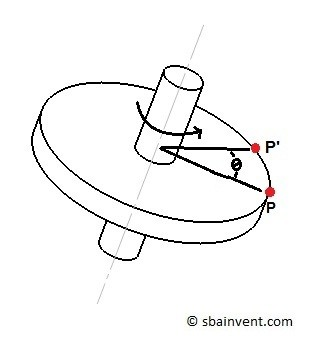
\includegraphics[scale=0.25]{fixed_axis_rot.jpg}
        \end{figure}
        \column{.45\textwidth}
    \end{columns}
    \vspace{5pt}
    $\to$ Rotational Symmetry
\end{frame}

\begin{frame}{Energy: What Moves You Through Time?}
    \begin{itemize}
        \item $K = \frac{1}{2}mv^2$
        \item $U$ is the ``potential energy''
        \item $F_j = - \frac{\partial}{\partial x^{\hspace{1pt}j}} U$ or: $\Vec{F} = - \nabla U$
    \end{itemize}
\end{frame}

\begin{frame}{Example: A Spinning Hoop}
    \begin{itemize}
        \item $\vec{F} = \vec{\textrm{?}}$
        \item what are the equilibria?
    \end{itemize}

    \begin{figure}
        \centering
        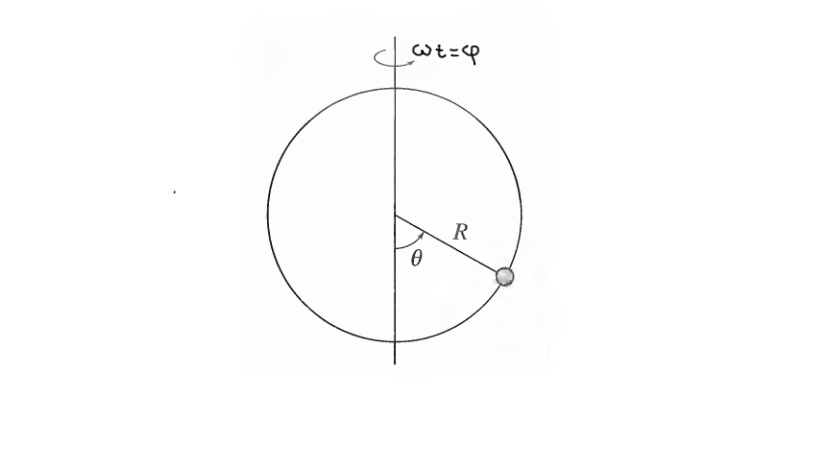
\includegraphics[scale=0.5]{bead_on_hoop.png}
        \label{fig:bead_on_hoop}
    \end{figure}
\end{frame}

\section{Lagrangian Mechanics}

\begin{frame}{Variational Principles}
\begin{columns}[c]

\column{0.5\textwidth}
    \begin{itemize}
        \item Shortest distance between two points?
        \item Two approaches: Local vs Global
        \begin{itemize}
            \item Newton's Laws
            \item Lagrangian Mechanics
        \end{itemize}
    \end{itemize}
    
\column{0.5\textwidth}
\begin{figure}
    \centering
    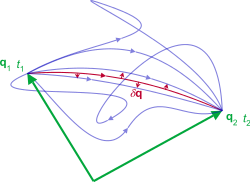
\includegraphics[scale=0.5]{least_action_paths.png}
    \label{fig:paths}
\end{figure}

\end{columns}
    
\end{frame}

\begin{frame}{What is a Lagrangian?}
    \begin{itemize}
        \item A \textbf{Lagrangian} is defined as $L = K - U$ \hfill $[L] = J$
        \item The \textbf{action} is $S = \int L dt$ \hfill $[S] = J\cdot s$
        \pause \item \textbf{Hamilton's Principle} says that the real path makes the action ``stationary''
        \vspace{90pt}
        \only<3>{$\frac{\partial L}{\partial q} - \dv{t} \frac{\partial L}{\partial \dot{q}}=0$ are the Euler Lagrange Equations}
    \end{itemize}
\end{frame}

\begin{frame}{Newton's Laws in Lagrangian Mechanics}
    \begin{itemize}
        \item $K = \frac{1}{2}m\dot{\Vec{q}} \cdot \dot{\Vec{q}} = \frac{1}{2} m\dot{q}^2$ where $\dot{q} = |\dot{\Vec{q}}|$
        \item $U = U(q)$
        %show EL eqns are newtons laws with L=K-U
        \pause\item Hamilton's Principle is \textbf{the exact same} as Newton's laws
        \item What if we chose a more general ``label'' than $x$?
    \end{itemize}

\end{frame}

\begin{frame}{Polar Coordinates}

\begin{itemize}
    \item $\dot{\Vec{r}} = \frac{d}{dt} \left((r \cos{\theta})\hat{x} + (r\sin{\theta}) \hat{y}\right) = (\dot{r} \cos{\theta} - r \dot{\theta} \sin{\theta})\hat{x} + (\dot{r}\sin{\theta} + r \dot{\theta} \cos{\theta}) \hat{y}$
    \item $K = \frac{m}{2}\dot{\Vec{r}} \cdot \dot{\Vec{r}} =\frac{m}{2} \left(\dot{r}^2 + r^2 \dot{\theta}^2\right)$
    %compute dL/dthetadot

\end{itemize}
    
\end{frame}

\begin{frame}{Polar Coordinates}

\begin{itemize}
    \item $\dot{\Vec{r}} = \frac{d}{dt} \left((r \cos{\theta})\hat{x} + (r\sin{\theta}) \hat{y}\right) = (\dot{r} \cos{\theta} - r \dot{\theta} \sin{\theta})\hat{x} + (\dot{r}\sin{\theta} + r \dot{\theta} \cos{\theta}) \hat{y}$
    \item $K = \frac{m}{2}\dot{\Vec{r}} \cdot \dot{\Vec{r}} =\frac{m}{2} \left(\dot{r}^2 + r^2 \dot{\theta}^2\right)$
    %compute dL/dthetadot
    \vspace{90pt}
    \item For any coordinate $q$, $\frac{\partial L}{\partial \dot{q}}$ is the \textbf{generalized momentum} associated to $q$
\end{itemize}

\end{frame}

\begin{frame}{Example: The Harmonic Oscillator}
\begin{itemize}
    \item $L = \frac{1}{2}m\dot{x}^2 - \frac{1}{2}kx^2$
\end{itemize}
    %do it
\end{frame}



\begin{frame}{Example: A Spinning Hoop}
    \begin{itemize}
        \item $L = \frac{1}{2}mR^2(\dot{\theta}^2 + \omega^2\sin^2{\theta}) - mgR(1-\cos{\theta})$ \newline
        \item $\frac{\partial L}{\vspace{1pt}\partial \dot{\theta}} = mR^2 \dot{\theta}$ \hspace{10pt}
        $\dv{t}\left(\frac{\partial L}{\partial \dot{\theta}}\right) = mR^2 \ddot{\theta}$ \hspace{10pt}$\pdv{L}{\theta} = mR^2 \omega^2 (\sin\theta \cos\theta) - mgR\sin\theta$ 
    \end{itemize}
    %do it
    \begin{figure}
        \hspace{-3in}
        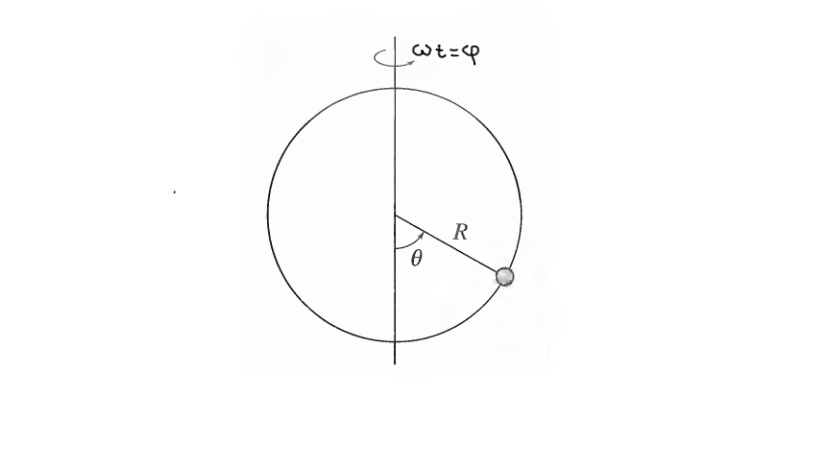
\includegraphics[scale=0.4]{bead_on_hoop.png}
        \label{fig:bead_on_hoop}
    \end{figure}
\end{frame}

\begin{frame}{A Note on Momentum}
    \begin{itemize}
        \item The EL Equations say that $\frac{d}{dt} p_j = \frac{\partial L}{\partial q^j}$
        \item So, if $L$ doesn't depend on $q^{\textrm{ }j}$ then $p_j$ is conserved!
    \end{itemize}
\end{frame}

\begin{frame}{Newton's Laws in the Lagrangian Formalism}
\begin{center}
\begin{tabular}{|c|c|}
    \hline
    Newton & Lagrange  \\
    \hline 
    Objects go in ``straight lines'' & Inertial Frames Exist \\
    $F = ma$ & Hamilton's Principle ($\delta S = 0$) \\
    Equal \& Opposite Reactions & Space is homogeneous\\
    \hline
\end{tabular}
\end{center}
\begin{itemize}
    \item Two about the setting, one about the physics!
\end{itemize}
\end{frame}

\section{Hamiltonian Mechanics}

\begin{frame}{What is a Hamiltonian?}
    \begin{itemize}
        \item We've seen that $p = \frac{\partial L}{\partial \dot{q}}$
        \item $L = p \dot{q} - H(q,p,t)$
        \item $H = p \dot{q} - L(q,p,t)$
        % show H = K + U normally (q = x etc)
    \end{itemize}
    
\end{frame}

\begin{frame}{What is a Hamiltonian?}
    \begin{itemize}
        \item $H = p \dot{q} - L(q,p,t)$
        \item $dL = \frac{\partial L}{\partial q}d q + \frac{\partial L}{\partial \dot{q}}d \dot{q}$
        % everything up till E-L substitution
        
        %\item $d(p \dot{q} - L) = dH = -\frac{\partial L}{\partial q}\delta q + \dot{q}dp $
        
        %\item $dH = -\frac{\partial L}{\partial q}  \delta q + \dot{q} dp $
    \end{itemize}
    
\end{frame}

\begin{frame}{What is a Hamiltonian?}
    \begin{itemize}
        \item $dH = -\frac{\partial L}{\partial q}  d q + \dot{q} dp $
        %EL eqns => first term is hamiltons eqns
    \end{itemize}
\end{frame}

\begin{frame}{Example: Hamiltonian of a Free Particle}
\begin{columns}[c]
    \column{.5\textwidth}
        \begin{itemize}
        \item $H = \frac{p^2}{2m}$
        %show that 1 2nd order becomes 2 1st order
        %introduce phase space
    \end{itemize}
    \column{.5\textwidth}
    \begin{figure}
        \centering
        \begin{tikzpicture}[scale=2.25]
        \draw[<->] (-1,0) -- (1,0);
        \draw[<->] (0,-1) -- (0,1);
        
        \node[anchor = west] at (0,1) {$p$};
        \node[anchor = west] at (1,0) {$q$};
        \end{tikzpicture}
        \label{fig:my_label}
    \end{figure}
\end{columns}

\end{frame}

\begin{frame}{Example: Hamiltonian of a Harmonic Oscillator}
        \begin{itemize}
            \item $H = \frac{p^2}{2m} + \frac{1}{2}kq^2 $
        \end{itemize}
\end{frame}

\begin{frame}{Example: Hamiltonian of a Harmonic Oscillator}
       \begin{itemize}
        \item $H = \frac{p^2}{2m} + \frac{1}{2}kq^2 = \frac{m}{2}\left(\left(\frac{p}{m}\right)^2 + (\omega q)^2 \right)$
        \end{itemize}
\end{frame}

\begin{frame}{$H =\frac{m}{2}\left(\left(\frac{p}{m}\right)^2 + (\omega q)^2 \right)$}
    \vspace{-10pt}
    \begin{figure}
        \begin{tikzpicture}[scale=2.25]
        \draw[<->] (-1,0) -- (1,0);
        \draw[<->] (0,-1) -- (0,1);
        
        \node[anchor = west] at (0,1) {$\frac{p}{m}$};
        \node[anchor = west] at (1,0) {$\omega q$};
        \end{tikzpicture}
        \label{fig:my_label}
    \end{figure}
\end{frame}

\begin{frame}{Hamiltonians and Energy}
    \begin{itemize}
        \item Understanding Hamiltonians helps us understand what energy actually is!
        \item An \textbf{observable} is any function $f(q,p)$ of position and momentum
        \pause \item $\frac{df}{dt} = \pdv{f}{t} + \pdv{f}{q}\dv{q}{t} + \pdv{f}{p}\dv{p}{t}$
    \end{itemize}
    %df/dt = df/dq qdot + df/dp pdot dt = {f,H} + \frac{\partial f}{\partial t}
    %easy way to show d/dt H = \partial / \partial t H
    %df/dx = {f,p} bc p "generates x translations"
    %H "generates time translations"
\end{frame}

\begin{frame}{Poisson Brackets}
    \begin{itemize}
        \item $\{A,B\} = \frac{\partial A}{\partial q} \frac{\partial B}{\partial p} - \frac{\partial A}{\partial p} \frac{\partial B}{\partial q} \hspace{20pt} \frac{df}{dt} = \frac{\partial f}{\partial t} + \{f,H\} \hspace{20pt} \frac{df}{dq} = \{f,p\}$
        \item $\frac{\partial H}{\partial p} = \frac{dq}{dt}$ \hspace{30pt} $-\frac{\partial H}{\partial q} = \frac{dp}{dt}$
    \end{itemize}
    % Hamiltons equations (and therefore EL equations) just a manifestation of dp/dt = {p,H} = -{H,p} = -dH/dq same w {H,q} (minus bc its a rotation of phase space, just like SHO)
\end{frame}

\begin{frame}{Poisson Brackets}
    \begin{itemize}
        \item $\{A,B\} = \frac{\partial A}{\partial q} \frac{\partial B}{\partial p} - \frac{\partial A}{\partial p} \frac{\partial B}{\partial q} \hspace{20pt} \frac{df}{dt} = \frac{\partial f}{\partial t} + \{f,H\} \hspace{20pt} \frac{df}{dq} = \frac{\partial f}{\partial q} + \{f,p\}$ \newline
        \item Bilinearity: $\{af+bg,h\} = a\{f,h\} + b\{g,h\}$ \newline
        \item Antisymmetry: $ \{A,B\} = - \{B, A\}$ \newline
        \item Jacobi Identity: $\{A, \{B, C\}\} + \{B, \{C, A\}\} + \{C, \{A, B\}\} = 0$
    \end{itemize}
    %properties of {,}, should we add these so its easier to neglect LOL
\end{frame}

\begin{frame}{Noether's Theorem Strikes Again!}
    \begin{itemize}
        \item Let's say that $\frac{df}{d a} = \{f,A\}$ and $\frac{df}{db} = \{f,B\}$
    \end{itemize}
    %in general df/d \epsilon = {f,g} if g generates epsilon transforms
    %df/dt = 0 iff {f,H} = 0 iff {H,f}= 0 iff dH/depsilon = 0
    % another example of noether: symm of H lead to conserved quantities and vice versa
\end{frame}

\section{Takeaways}

\begin{frame}{Takeaways}

\begin{itemize}
    \item There are many possible ``fundamental'' ways to formulate even classical mechanics
    \item Symmetry and geometry can lead to deep physics!
    \item Question: the Hamiltonian generates time translations, momentum generates space translation. What does this tell us about the true nature of energy?
\end{itemize}

    \hspace{100pt}
    
    \begin{figure}
    \centering
    \def\omu{13}
    \def\oml{-7}
    \begin{tikzpicture}
    
    %labels
    \node[anchor=south] at (-5,0.1) {\small $26$};
    \node[anchor=south] at (-0.1639*\omu-0.7377,0.1) {\small $\omu$};
    \node[anchor=north] at (-0.1639*\oml-0.7377,-0.1) {\small $\oml$};
    \node[anchor=north] at (5,-0.1) {\small $-35$};
    
    %blue fill bar
    \filldraw (-5,0) -- (-0.1639*\omu-0.7377,0);
    %red fill bar
    \filldraw[red] (-0.1639*\omu-0.7377,-0.1) --  (-0.1639*\omu-0.7377,0.1) -- (-0.1639*\oml-0.7377,0.1)--(-0.1639*\oml-0.7377,-0.1) -- cycle;
    %blue thin bar
    \draw[thick] (-0.1639*\oml-0.731,0) -- (5,0);
    %vertical blue thin bar
    \draw[thick] (5,.1) -- (5,-.1);
    \draw[thick] (-5,.1) -- (-5,-.1);
    %1m mark
    \draw[thick, orange] (-0.7377,.1) -- (-0.7377,-.1);

    \end{tikzpicture}
    \label{fig:progress}
\end{figure}

\end{frame}

\begin{frame}{Takeaways}

\begin{itemize}
    \item There are many possible ``fundamental'' ways to formulate even classical mechanics
    \item Symmetry and geometry can lead to deep physics!
    \item Question: the Hamiltonian generates time translations, momentum generates space translation. What does this tell us about the true nature of energy?
\end{itemize}

    \hspace{100pt}
    
    \begin{figure}
    \centering
    \def\omu{26}
    \def\oml{-35}
    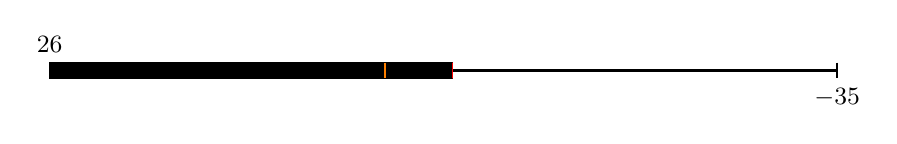
\begin{tikzpicture}
    
    %labels
    \node[anchor=south] at (-5,0.1) {\small $26$};
    \node[anchor=south] at (-0.1639*\omu-0.7377,0.1) {\small $\omu$};
    \node[anchor=north] at (-0.1639*\oml-0.7377,-0.1) {\small $\oml$};
    \node[anchor=north] at (5,-0.1) {\small $-35$};
    
    %blue fill bar
    \filldraw (-5,0.1) -- (-0.1639*\omu-0.7377,0.1) -- (-0.1639*\omu-0.7377,-0.1) -- (-5,-0.1) -- cycle;
    %red fill bar
    \filldraw[red] (-0.1639*\omu-0.7377,-0.1) --  (-0.1639*\omu-0.7377,0.1) -- (-0.1639*\oml-0.7377,0.1)--(-0.1639*\oml-0.7377,-0.1) -- cycle;
    %blue thin bar
    \draw[thick] (-0.1639*\oml-0.731,0) -- (5,0);
    %vertical blue thin bar
    \draw[thick] (5,.1) -- (5,-.1);
    \draw[thick] (-5,.1) -- (-5,-.1);
    %1m mark
    \draw[thick, orange] (-0.7377,.1) -- (-0.7377,-.1);

    \end{tikzpicture}
    \label{fig:progress}
\end{figure}
    
\end{frame}

\end{document}